\documentclass{article}
\usepackage{amsmath}
\usepackage{amssymb}
\usepackage[margin=.5in]{geometry}
\usepackage{array} 
\usepackage{tikz}
\usetikzlibrary{shapes, arrows.meta} 
\newcommand{\tuple}[1]{\ensuremath{\left\langle #1 \right\rangle}}
\newcommand{\pare}[1]{ \left( #1 \right) }
\newcommand{\justify}[1]{%
  \begin{equation*}
  \begin{aligned}
  & #1
  \end{aligned}
  \end{equation*}
}

\begin{document}
    
\textbf{Exercice 2}

\vspace{0.3cm}
A) a) 

1) $\mathcal{R}$ est réflexive car elle contient l'identité. Vérifions l'antisymétrie. Pour les éléments $\tuple{1,4}, \tuple{3,2},$ et $\tuple{4,5}$, 

l'antisymétrie est trivialement vraie car $\mathcal{R}$ ne contient pas $\tuple{4,1}, \tuple{2,3},$ et $\tuple{5,4}$. Pour les paires identitaires 

$\tuple{1, 1}, \tuple{2, 2}, \tuple{3, 3}, \tuple{4, 4}, \tuple{5, 5} \in \mathcal{R}$, l'antisymétrie est évidemment satisfaite. Cependant, $\mathcal{R}$ n'est pas transitive car 

$$ \tuple{1,4} \land \tuple{4,5} \in \mathcal{R}$$

et pourtant $ \tuple{1,5} \notin \mathcal{R}.$ Ainsi, ce n'est pas un ordre partiel, et nous ne pouvons pas construire un diagramme de Hasse.

\vspace{0.5cm}

2)
Ceci n'est pas une relation d'équivalence non plus car, comme nous l'avons vu en 1), elle n'est pas transitive. De 

plus, elle n'est pas symétrique, ce qui est également requis pour une relation d'équivalence. En effet,

$$ \tuple{1,4} \in \mathcal{R} \land \tuple{4,1} \notin \mathcal{R}$$

\vspace{0.5cm}

b) 1) Calculons $\mathcal{R} \circ \mathcal{R}$ en ignorant les paires symétriques puisqu'elles sont redondantes. Nous obtenons 

$$ \tuple{1,4} \circ \tuple{4,5} = \tuple{1,5} $$

Ainsi, $$ \mathcal{R} \circ \mathcal{R} = \{ \tuple{1,5} \}$$

Par consequant $\mathcal{R}^+ = \mathcal{R} \cup \mathcal{R}^2 $ car ce sont les seules paires pour lesquelles la transitivité pouvait échouer. Nous avons 

maintenant un ordre partiel. Construisons le diagramme de Hasse.

\begin{center}
    \begin{minipage}{0.3\textwidth}
        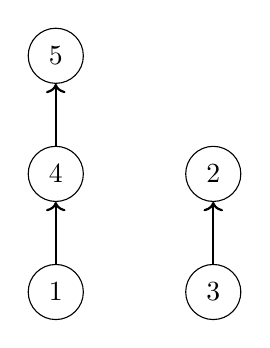
\begin{tikzpicture}
            \node[circle, draw, minimum size=0.7cm] (n1) at (0, -0.5) {1};
            \node[circle, draw, minimum size=0.7cm] (n4) at (0, 1) {4};
            \node[circle, draw, minimum size=0.7cm] (n5) at (0, 2.5) {5};
            \node[circle, draw, minimum size=0.7cm] (n3) at (2, -0.5) {3};
            \node[circle, draw, minimum size=0.7cm] (n2) at (2, 1) {2};

            \draw[->, thick] (n1) -- (n4);
            \draw[->, thick] (n4) -- (n5);
            \draw[->, thick] (n3) -- (n2);
        \end{tikzpicture}
    \end{minipage}
\end{center}

2) Cependant, la relation n’est toujours pas une relation d’équivalence car elle ne contient toujours pas la paire  $\tuple{4,1}$ et 

la symétrie échoue toujours.

\vspace{0.3cm}

c) 1)
Calculons l'inverse de $\mathcal{R}^{+}$ nous ignorons encore une fois les paires d'identités car elles servent de leur propre inverse
$$ \{ \tuple{1,4}^{-1},\tuple{3,2}^{-1},\tuple{4,5}^{-1},\tuple{1,5}^{-1} \} = 
\{ \tuple{4,1},\tuple{2,3},\tuple{5,4},\tuple{5,1} \}
$$

Donc,
$$ \mathcal{R}^{+} \cup (\mathcal{R}^{+})^{-1} = I_{\{1,2,3,4,5\}}\cup \{ \tuple{1,4},\tuple{3,2},\tuple{4,5},\tuple{1,5} 
\tuple{4,1},\tuple{2,3},\tuple{5,4},\tuple{5,1} \}.
$$

Conduisant clairement à un échec pur et simple de l'antisymétrie, $\mathcal{R}^{+} \cup (\mathcal{R}^{+})^{-1}$ n'est donc pas un ordre partiel.

2) Nous avons cependant maintenant une relation d'équivalence. $\mathcal{R}^{+} \cup (\mathcal{R}^{+})^{-1}$ partitions $ \{ 1,2,3,4,5 \}$ comme
$$\{ \{ 1,4,5 \} ,\{ 2,3 \} \}$$


effectivement, en considérant les éléments comme équivalents à l'intérieur des sous-ensembles. Nous pouvons représenter 

les classes comme $ [1]_{\mathcal{R}^{+} \cup (\mathcal{R}^{+})^{-1}} $ et $ [2]_{\mathcal{R}^{+} \cup (\mathcal{R}^{+})^{-1}} $

\vspace{0.3cm}

d) Si l'on reprenait la fermeture transitive, les images des paires composés avec l'ensemble lui-même conduiraient au 

même ensemble puisque la relation est déjà transitive. Cette relation est donc en fait la même que celle de c) 

$$(\mathcal{R}^{+} \cup (\mathcal{R}^{+})^{-1})^+ = \mathcal{R}^{+} \cup (\mathcal{R}^{+})^{-1}$$


\end{document}
